% set documentclass to widescree 16:9 ratio
\documentclass[aspectratio=169]{beamer}

% Load UofC_dynamic style file
\usepackage{UofC_dynamic}

% Title and author data
\title{Recurrent Spiking Neural Networks for EEG Decoding} %Title
\subtitle{Towards reliable BCI} %Subtitle
% Had to use \texorpdfstring{//} to ensure new line in presenter details
\author[]{Lex Berezowsk, Amirsaeed Ghodsinejad, Pahansith Kiriwaththuduwage\\  \texorpdfstring{\\} % presenter info
        \texorpdfstring{\\}
        Group 11}
\date{\today} % date

\begin{document}

%------------------------------------------------------------------------------------------------
\CustomTitlePage


%------------------------------------------------------------------------------------------------
\begin{frame}{Motivation}

    \begin{columns}[c]

        % Left column: Text
        \begin{column}{0.52\textwidth}
            \begin{itemize}
                \item Independent control of assistive devices for people with mobility impairments.
                \item Motor imagery as a control signal.
                \item Low EEG decoding accuracy remains a major barrier.
            \end{itemize}
        \end{column}

        % Right column: Image
        \begin{column}{0.45\textwidth}
            \centering
            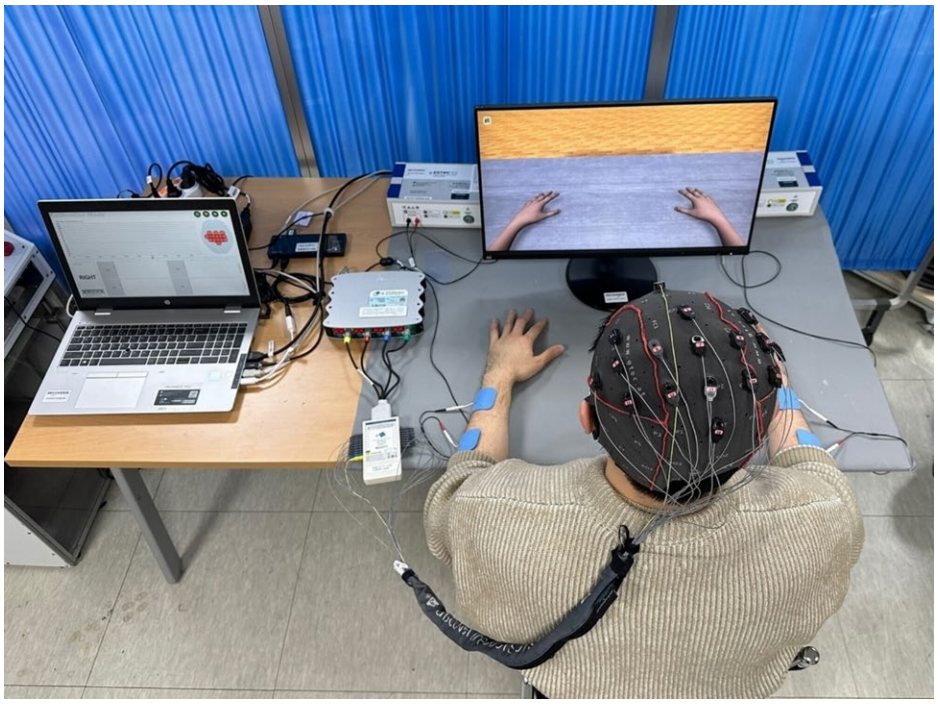
\includegraphics[width=\linewidth,
            height=6cm,keepaspectratio]{Images/BCI.png}
        \end{column}

    \end{columns}

\end{frame}

%------------------------------------------------------------------------------------------------

\begin{SplitFrame}{Existing EEG Decoding Approaches}

    \small
    \textbf{Artificial Neural Networks (ANN)}

    \textit{Example: EEGNet}

    \begin{center}
        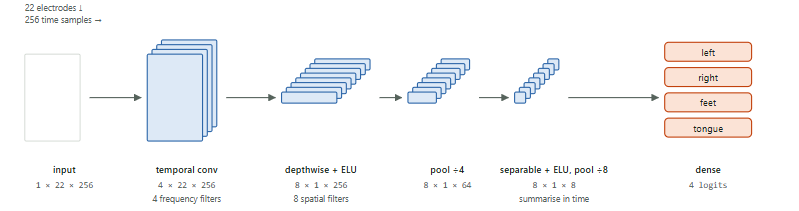
\includegraphics[width=0.95\linewidth,
        height=3cm,keepaspectratio]{Images/EEGNet.png}
    \end{center}

    \begin{itemize}
        \item Dedicated layers to extract temporal and spatial EEG features
    \end{itemize}

    \nextcolumn

    \small
    \textbf{FF-Spiking Neural Networks (SNNs)}

    \textit{Example: Converted EEGNet}

    \begin{center}
        \includegraphics[width=0.95\linewidth,
        height=3cm,keepaspectratio]{Images/SNN.png}
    \end{center}

    \begin{itemize}
        \item Neuron dynamics closer to those of biological neurons
    \end{itemize}

\end{SplitFrame}


%------------------------------------------------------------------------------------------------

\begin{frame}{Research Question/Gap}
    \small
    \begin{itemize}
        \item EEG originates from the collective activity of recurrently connected cortical neurons.
        \item Feedforward SNNs lack recurrent connections between neurons, limiting their ability to mimic these biological dynamics.
        \item RSNNs could exploit these dynamics to extract temporal features from EEG signals.
    \end{itemize}
    \begin{center}
        \large
        \centering
        \textbf{Can One Recurrent Spiking Layer Replace Dedicated Spatial and Temporal Filters for Cross-Session Motor Imagery EEG Decoding?}
    \end{center}
\end{frame}

%------------------------------------------------------------------------------------------------

% \begin{frame}{Research Question} 

% \large
% \centering
% \textbf{Can One Recurrent Spiking Layer Replace Dedicated Spatial and Temporal Filters for Cross-Session Motor Imagery EEG Decoding?}

% \end{frame}

%------------------------------------------------------------------------------------------------

\begin{frame}{The Dataset}
    
    \begin{center}
        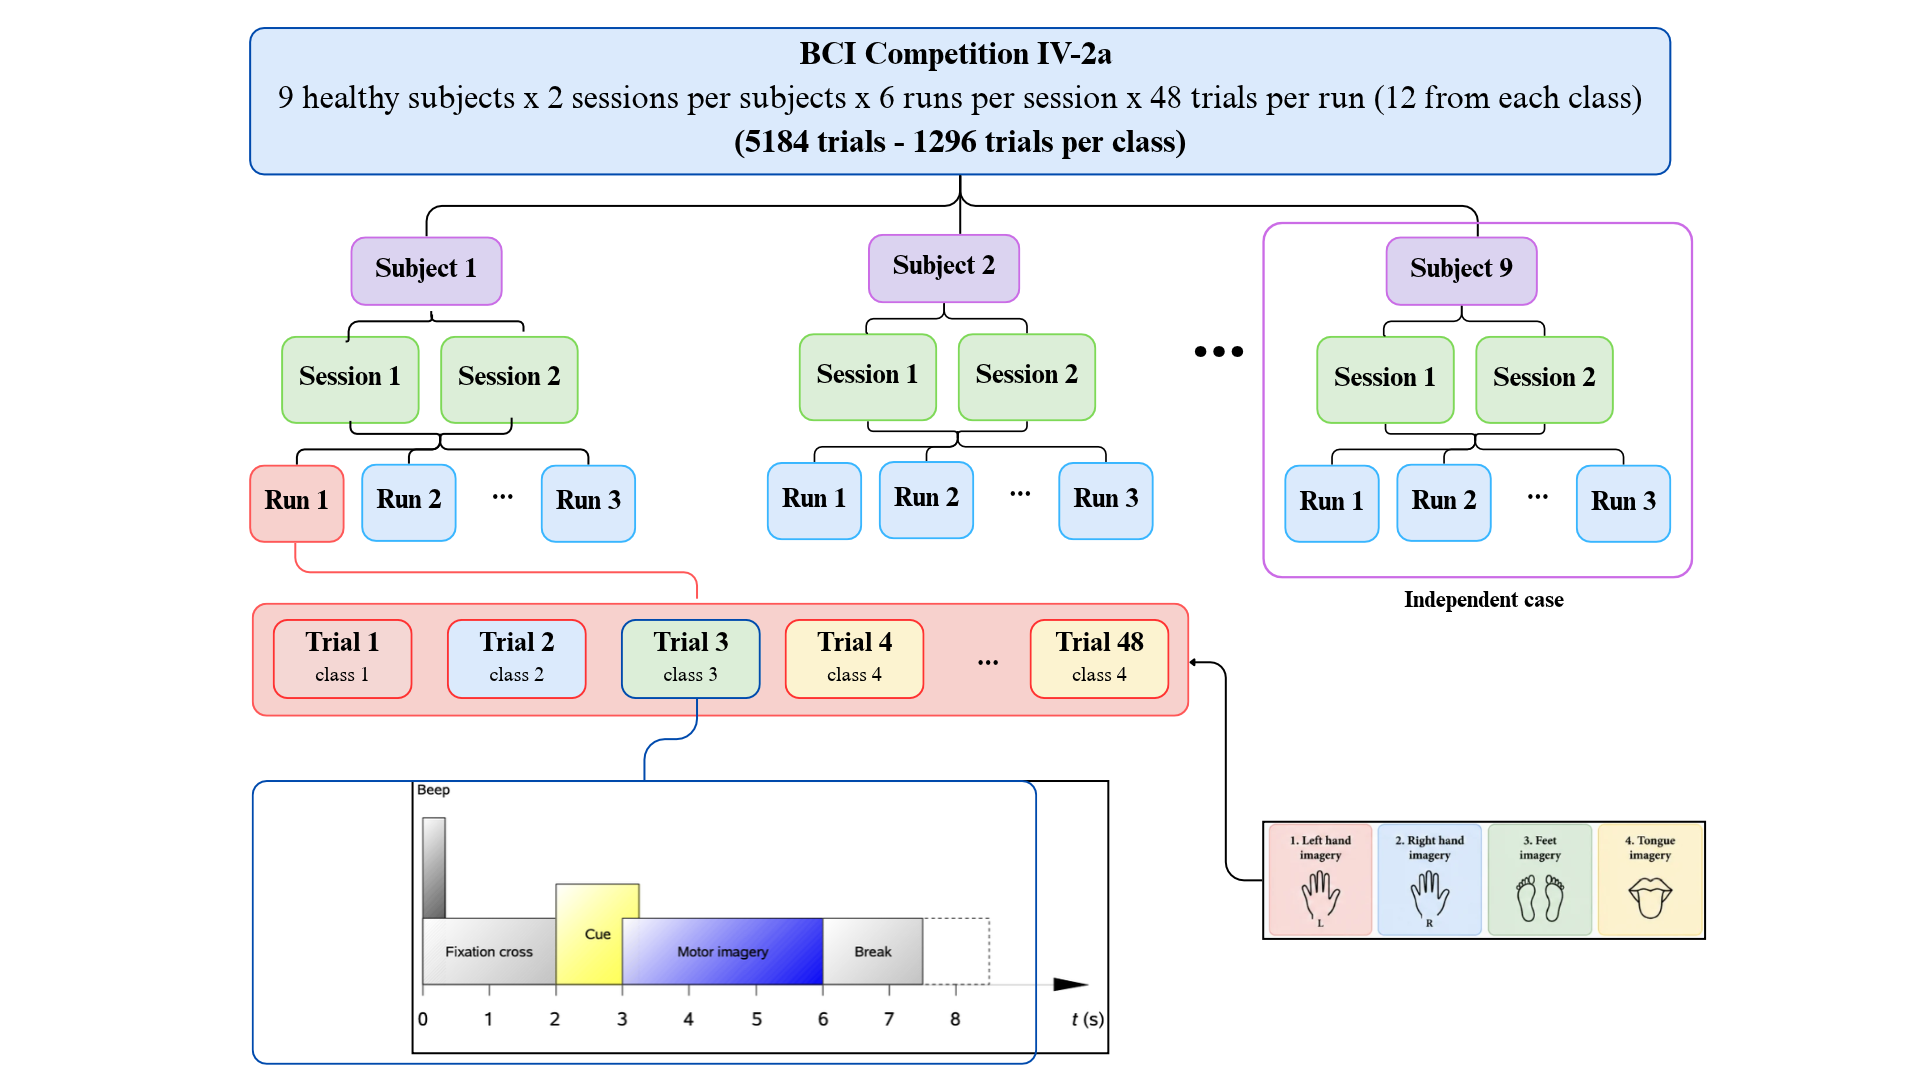
\includegraphics[width=0.95\linewidth,
        height=6.7cm,keepaspectratio]{Images/dataset_description.png}
    \end{center}
\end{frame}



%------------------------------------------------------------------------------------------------

\begin{frame}{Analysis Workflow}
    
    \begin{center}
        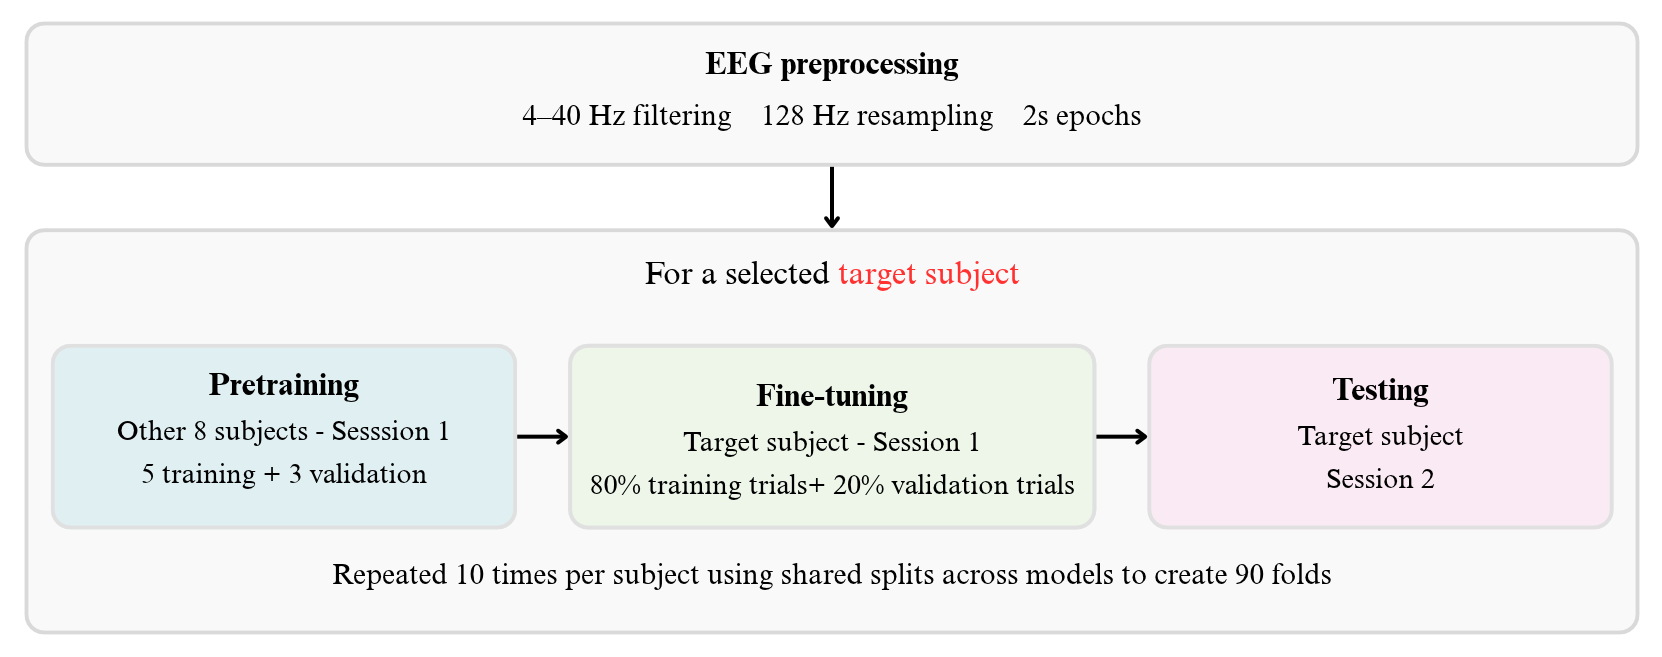
\includegraphics[width=0.95\linewidth,
        height=6.7cm,keepaspectratio]{Images/analysis_workflow.png}
    \end{center}
\end{frame}



%------------------------------------------------------------------------------------------------

\begin{frame}{Model Comparison}
    
    \begin{center}
        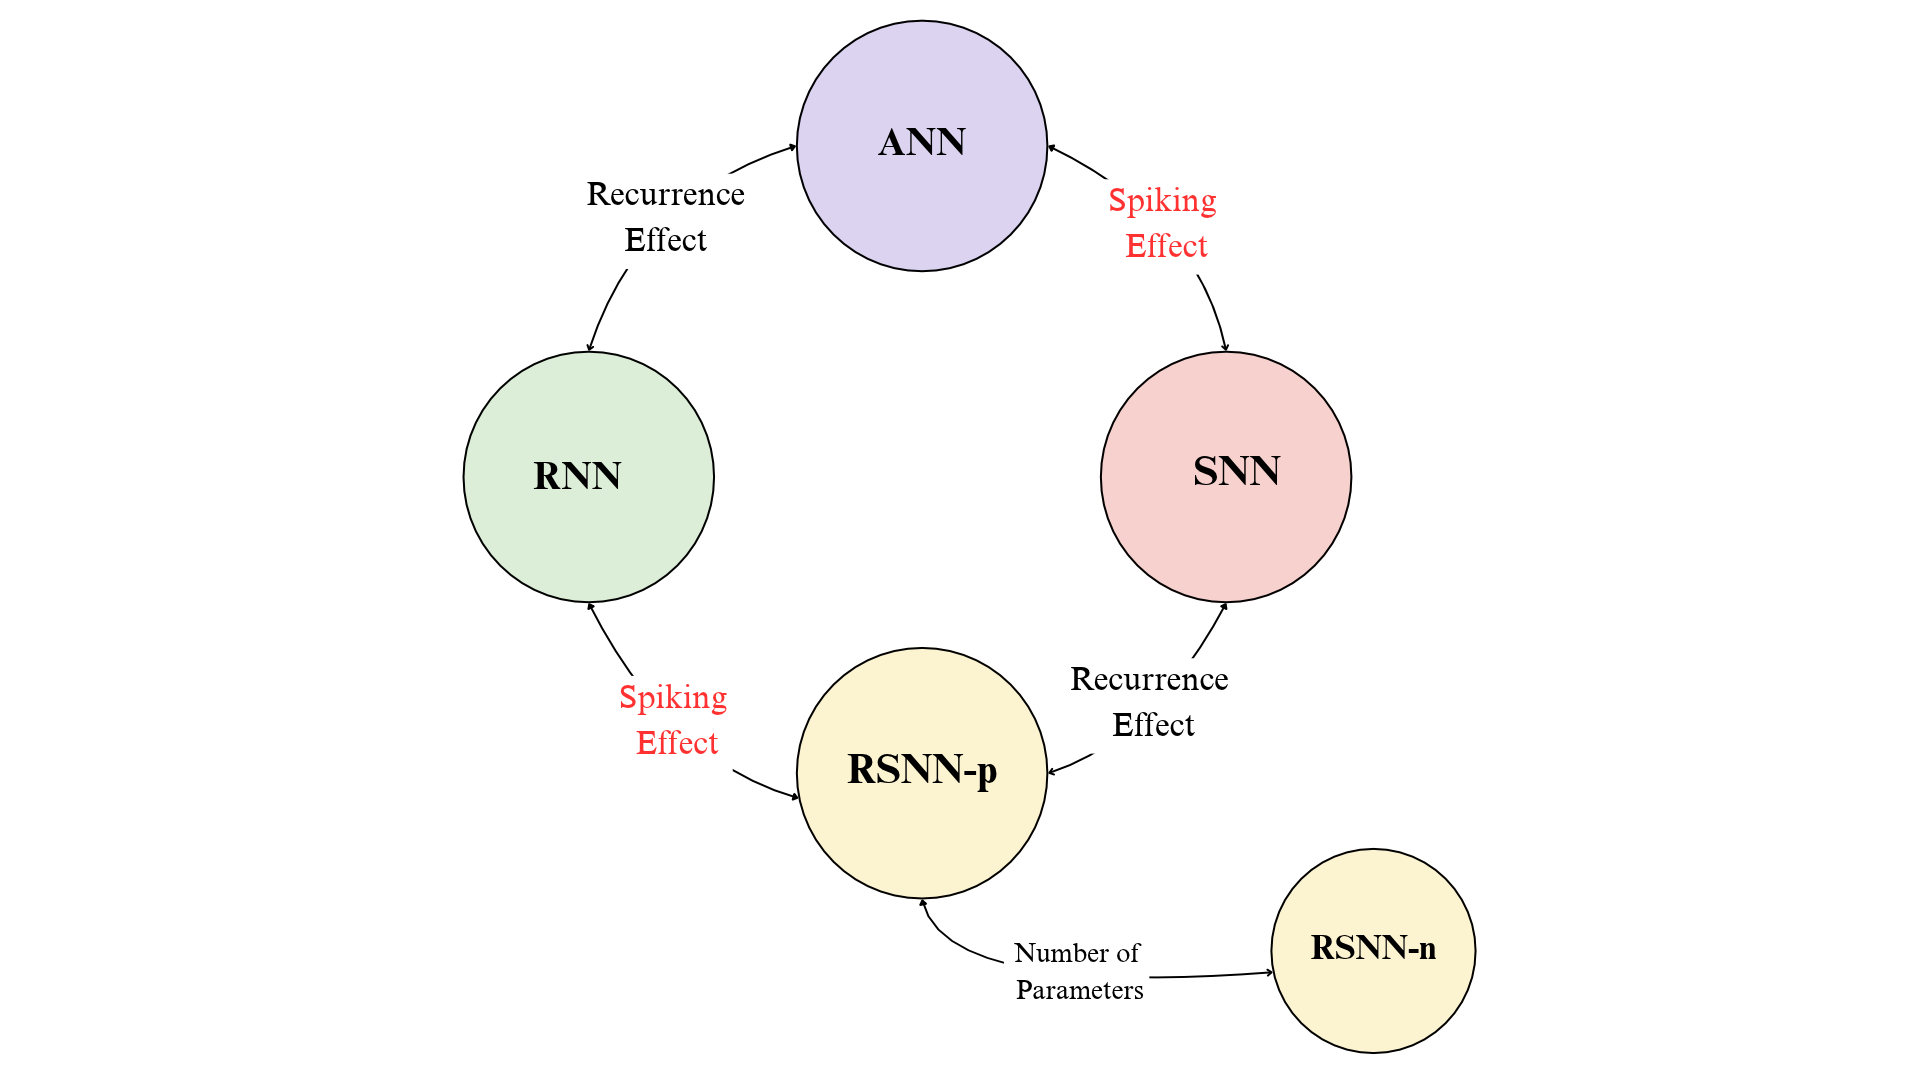
\includegraphics[width=0.95\linewidth,
        height=6.7cm,keepaspectratio]{Images/model_comparison.png}
    \end{center}
\end{frame}


%------------------------------------------------------------------------------------------------

\begin{frame}{Results}

    \begin{columns}[T]

        \begin{column}{0.69\textwidth}
            \centering
            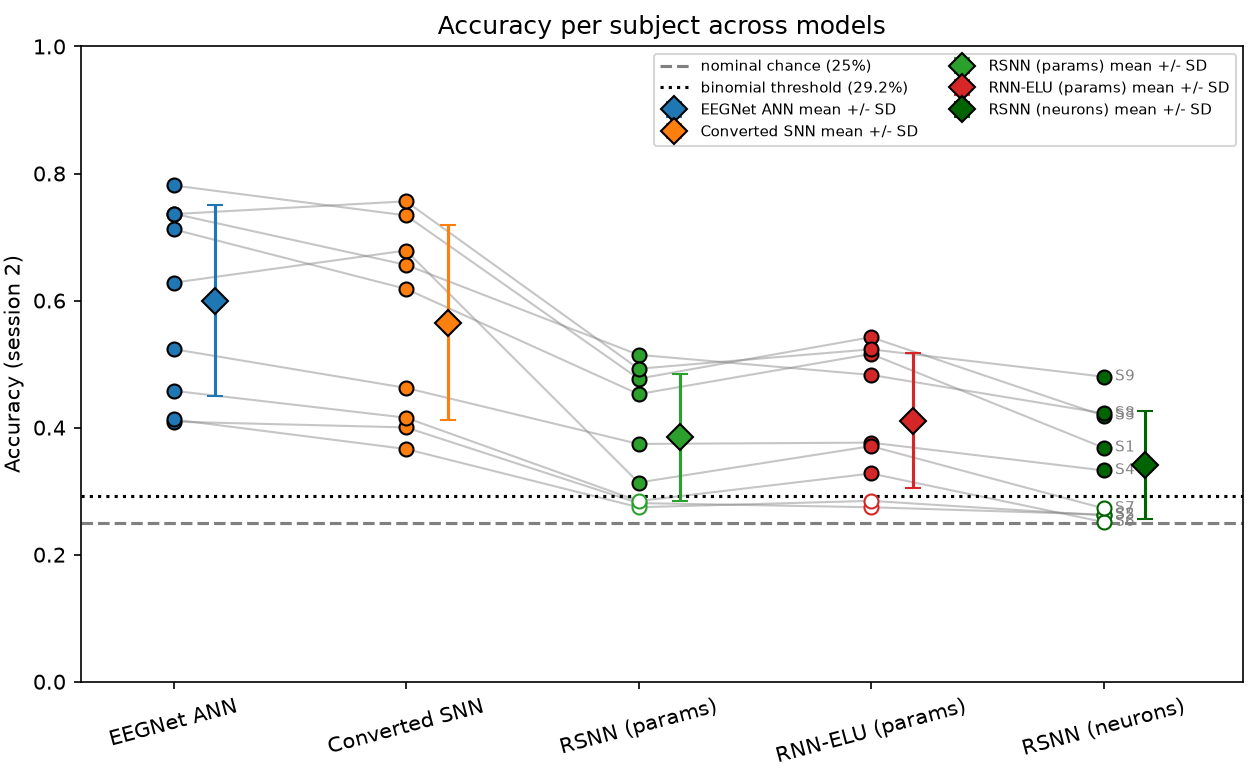
\includegraphics[width=\linewidth,
            height=6.7cm,keepaspectratio]
            {Images/accuracy_per_model.png}
        \end{column}

        \begin{column}{0.43\textwidth}
            \centering
            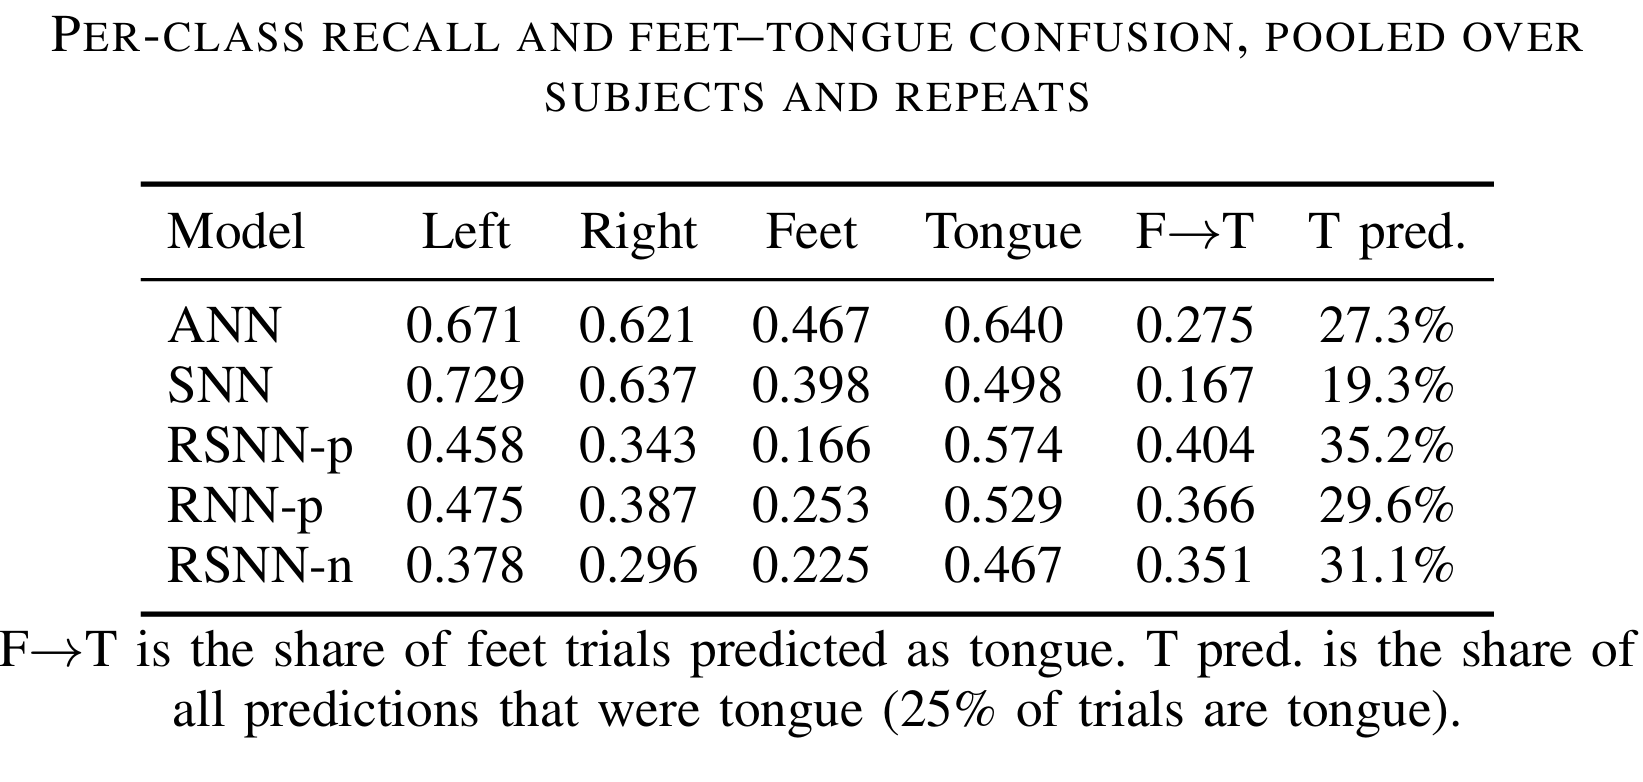
\includegraphics[width=\linewidth,
            height=6.7cm,keepaspectratio]
            {Images/class_wise_accuracy_table.png}
        \end{column}

    \end{columns}

\end{frame}



%------------------------------------------------------------------------------------------------

\begin{frame}{Limitations and Future Works}
    
    \small
        \begin{itemize}
            \item Limitations
                \begin{itemize}
                    \item Hyperparameters selected for EEGNet rather than RSNNs.
                    \item Individual contributions of intra- and inter-recurrence not isolated.
                    \item Limited exploration of network sizes.
                    \item Small sample size and offline evaluation.
                    \item Energy efficiency not evaluated.
                \end{itemize}
            \item Future Works
                \begin{itemize}
                    \item Optimize RSNN-specific hyperparameters.
                    \item Investigate intra- and inter-recurrence separately.
                    \item Introduce learnable transmission delays to improve temporal feature extraction.
                    \item Validate using larger, clinically relevant datasets.
                    \item Evaluate energy efficiency and real-time performance.
                \end{itemize}
        \end{itemize}

    
\end{frame}

%------------------------------------------------------------------------------------------------

\begin{frame}{Final Interpretation }

\Large
\centering
A single recurrent spiking layer did not match EEGNet under the investigated conditions.The recurrent feature extraction design appears to be a greater limitation than spiking itself.

\end{frame}

%------------------------------------------------------------------------------------------------

\ThankYouFrame{
    Thank you!
}{
    \small
    GitHub Repository:  \url{https://github.com/thesixtium/bmen-600-group-11}
}{
    \small
    Lex Berezowsk, Amirsaeed Ghodsinejad, Pahansith Kiriwaththuduwage\\
    Group 11
}



%------------------------------------------------------------------------------------------------

\begin{frame}{The Dataset}
    
    \small
        \begin{itemize}
            \item No subject or trial was excluded. 
            \item Trials marked by the dataset’s expert as containing artifacts were kept, leaving \textbf{72 trials per class in every session}. 
            \item A class-specific band-power changes in the data demonstrated the quality and ability to use the dataset. 
        \end{itemize}
        \begin{center}
            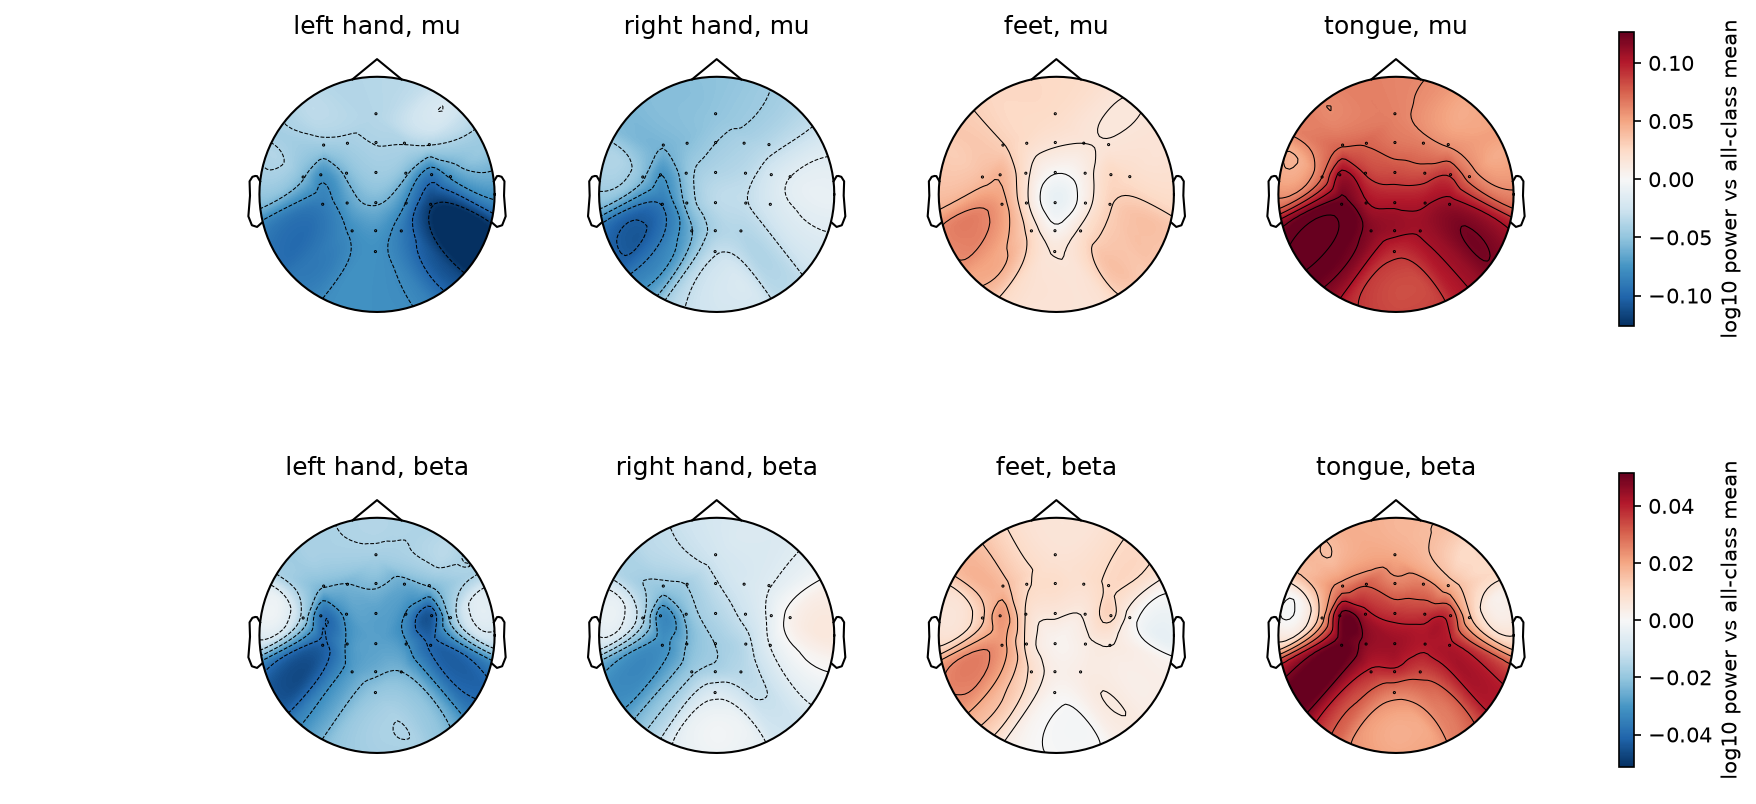
\includegraphics[width=0.95\linewidth,
            height=4.5cm,keepaspectratio]{Images/class_topomaps.png}
        \end{center}
    
\end{frame}

%------------------------------------------------------------------------------------------------

\begin{frame}{Analysis Workflow}
    
    \begin{center}
        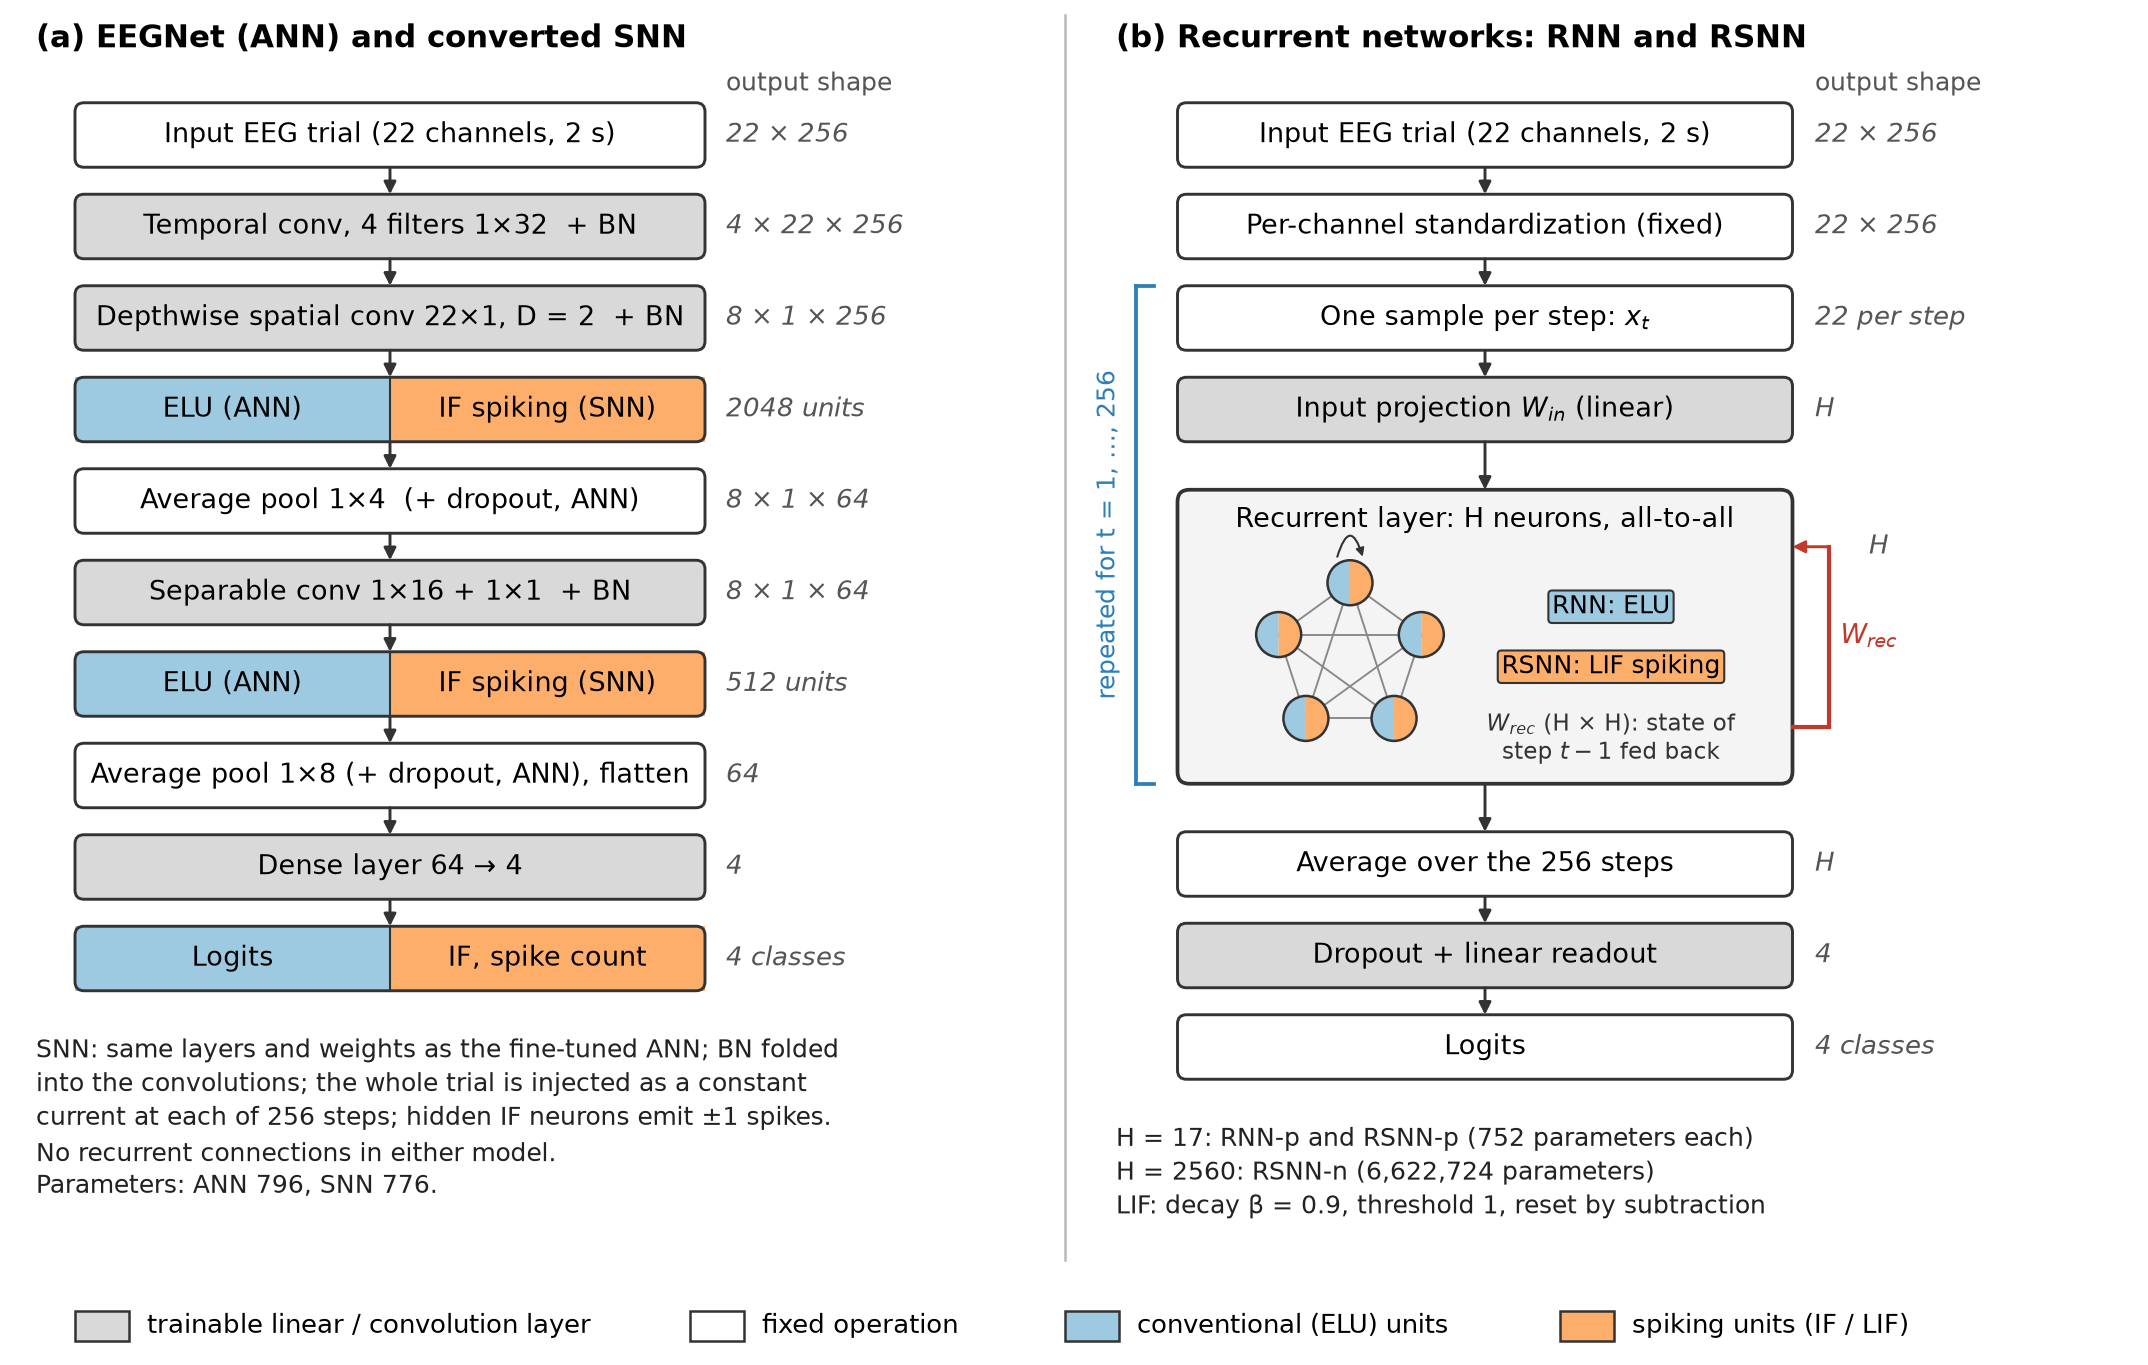
\includegraphics[width=0.95\linewidth,
        height=6.7cm,keepaspectratio]{Images/model_architectures.png}
    \end{center}
\end{frame}

%------------------------------------------------------------------------------------------------

\begin{frame}{Results}
    
    \begin{center}
        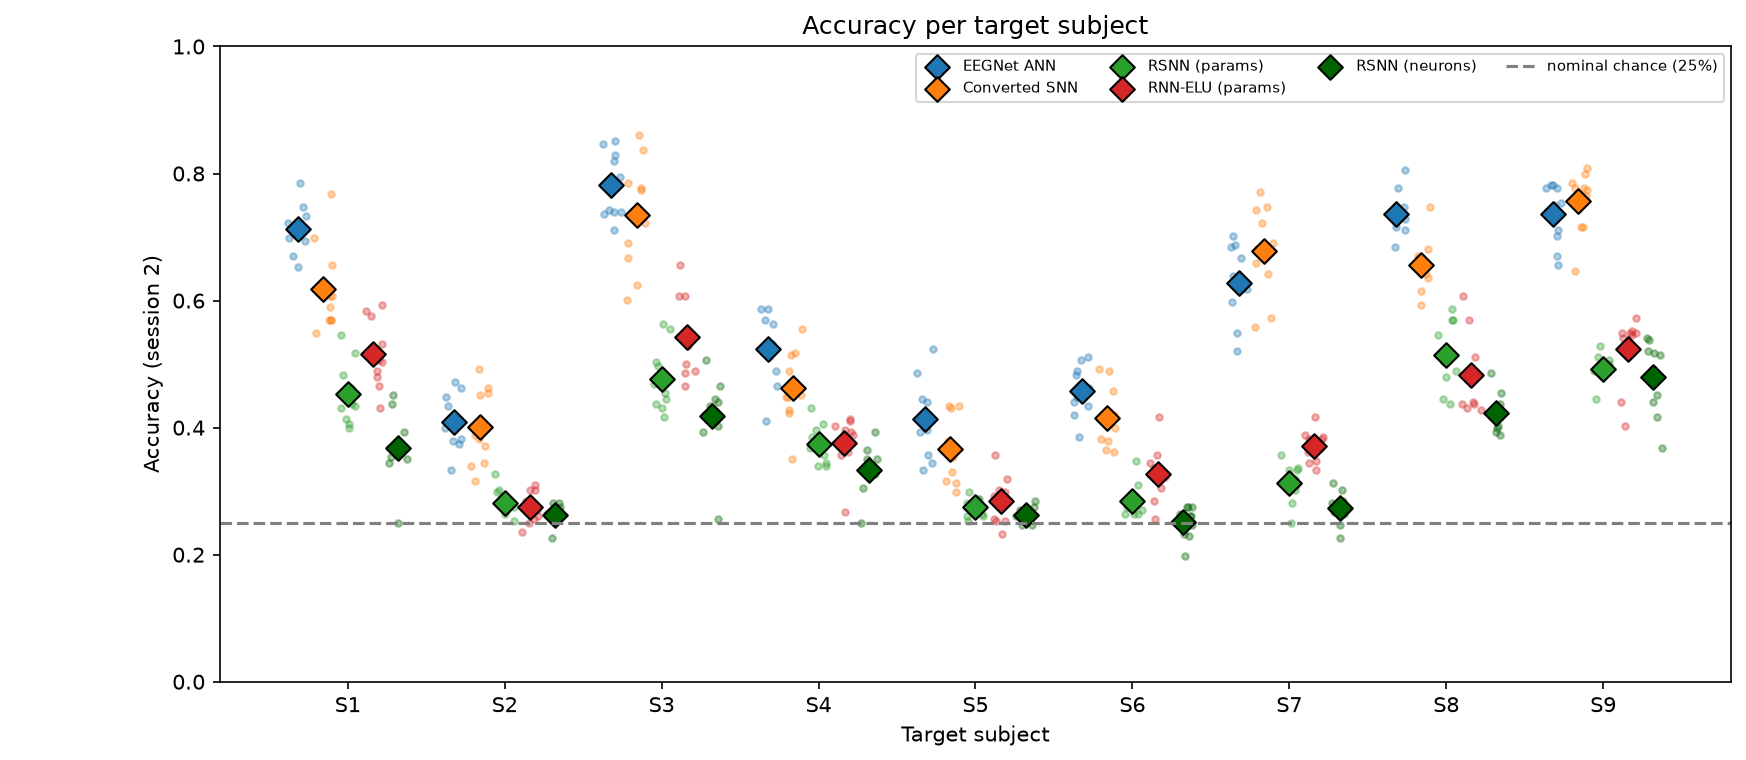
\includegraphics[width=0.95\linewidth,
        height=6.7cm,keepaspectratio]{Images/accuracy_per_subject.png}
    \end{center}
\end{frame}

%------------------------------------------------------------------------------------------------

\begin{frame}{Results}
    
    \begin{center}
        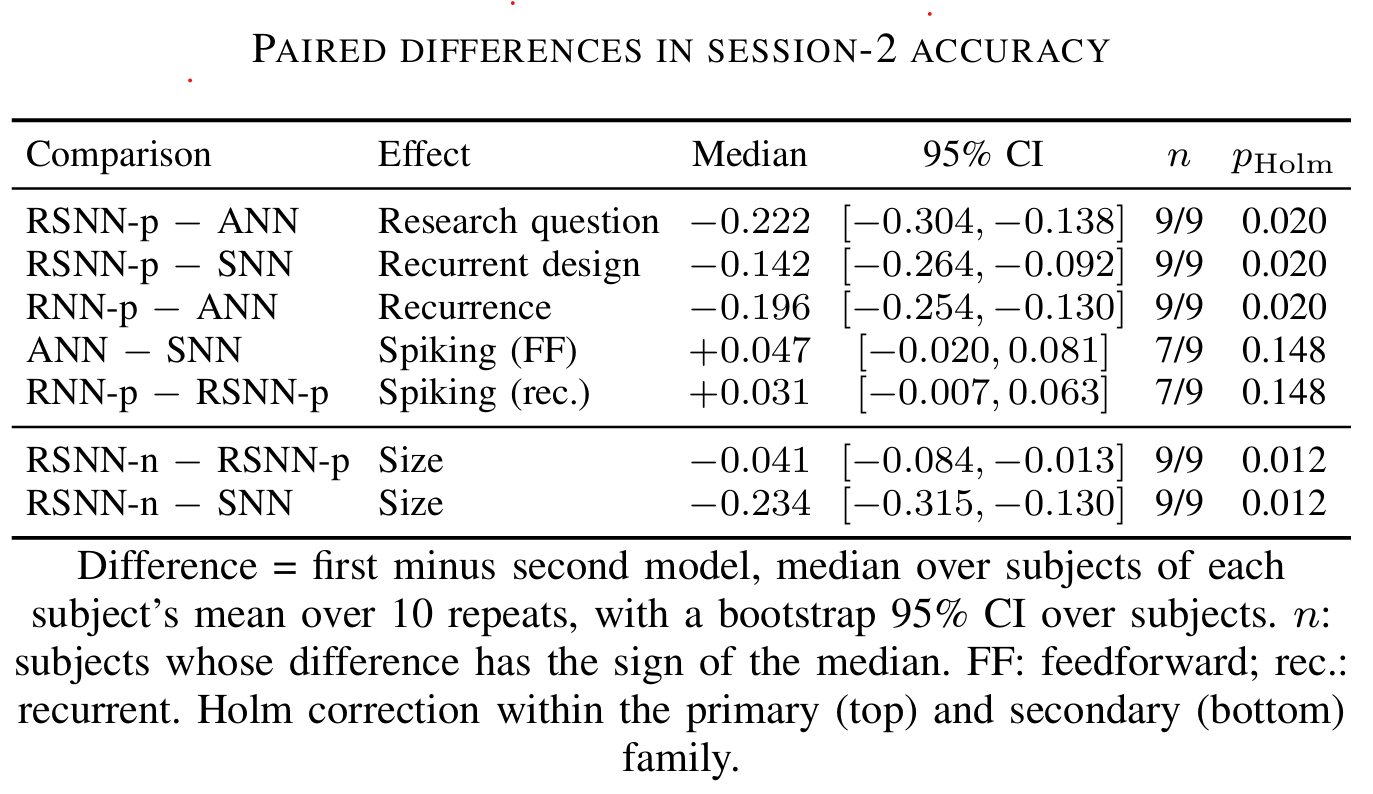
\includegraphics[width=0.95\linewidth,
        height=6.7cm,keepaspectratio]{Images/model_comparison_accuracy_table.png}
    \end{center}
\end{frame}

\end{document}
